\documentclass[handout, 9pt]{beamer}

%!TEX root = ../notas_de_clase.tex

%preamble

%language
\usepackage[spanish,es-nodecimaldot]{babel}
\usepackage[utf8]{inputenc}
\usepackage{apacite}
\usepackage[absolute,overlay]{textpos}

%packages
\usepackage[Algoritmo]{algorithm}
\usepackage{algorithmicx}
\usepackage[noend]{algpseudocode}
\usepackage{mathtools}
\setlength {\marginparwidth}{2cm}
\usepackage{todonotes}
\usepackage{amsbsy}
\usepackage{amssymb}
\usepackage{amsmath,bm}
\usepackage{dsfont}

\usepackage{xcolor}
\providecommand{\sred}[1]{\textcolor{red}{#1}}
\providecommand{\sblue}[1]{\textcolor{blue}{#1}}
\providecommand{\red}[1]{\textcolor{red}{\text{#1}}}
\providecommand{\blue}[1]{\textcolor{blue}{\text{#1}}}
\providecommand{\redb}[1]{\textcolor{red}{\textbf{#1}}}
\providecommand{\blueb}[1]{\textcolor{blue}{\textbf{#1}}}
\usepackage{graphicx}
\usepackage{fancybox}
\usepackage{booktabs}
\usepackage{caption}
\usepackage{float}
%\usepackage[longend,ruled,algochapter,linesnumbered,lined,boxed,commentsnumbered,spanish]{algorithm2e}
%\usepackage[algo2e]{algorithm2e}
\usepackage{amssymb}
\usepackage{amstext}
\usepackage{bm}
\usepackage{wrapfig}
\usepackage{subcaption} % para_unsupervised_chapter

%formatting

\usepackage[export]{adjustbox}

%caption para figuras
\captionsetup[figure]{width=.8\linewidth, font=small,labelfont={bf},name={Fig.},labelsep=period}
\captionsetup[table]{width=.8\linewidth,font=small,labelfont={bf},name={Tabla},labelsep=period}



\ifx\byn\undefined
    \definecolor{my_blue}{HTML}{C2D5FF}
    \definecolor{my_red}{HTML}{FFC2C2}
    \definecolor{my_yellow}{HTML}{FFFFE0}
\else
    \definecolor{my_blue}{HTML}{FFFFFF}
    \definecolor{my_red}{HTML}{FFFFFF}
    \definecolor{my_yellow}{HTML}{FFFFFF}
\fi


\usepackage[framemethod=TikZ]{mdframed}
\mdfdefinestyle{discusion}{%
    %linecolor=black,
    %outerlinewidth=0pt,
    roundcorner=0pt,
    innertopmargin=5pt,
    innerbottommargin=5pt,
    innerrightmargin=20pt,
    innerleftmargin=20pt,
    backgroundcolor=my_blue}

\colorlet{Green}{green!90}


\mdfdefinestyle{ejemplo}{%
    %linecolor=black,
    %outerlinewidth=0pt,
    roundcorner=0pt,
    innertopmargin=5pt,
    innerbottommargin=5pt,
    innerrightmargin=20pt,
    innerleftmargin=20pt,
    backgroundcolor=my_yellow}


\mdfdefinestyle{pendiente}{%
    style = discusion, 
    backgroundcolor=my_red}


\RequirePackage{url}



%definitions
\def\td{{\text d}}
\def\cN{{\mathcal N}}
\def\cX{{\mathcal X}} 
\def\cC{{\mathcal C}} 
\def\N{{\mathbb N}}
\def\d{{\text d}}
\def\datos{{\mathcal D}}
\def\eye{{\mathbb I}}
\def\ssum{{\scriptstyle\sum}}
\def\bepsilon{{\bm \epsilon}}
\def\tx{\tilde{x}}
\def\tX{\tilde{X}}
\def\thetaMAP{\theta_\text{MAP}}
\newcommand{\gp}{\ensuremath{\mathcal{GP}}}
\newcommand{\pr}{\ensuremath{\mathbb{P}}}
\newcommand{\x}{\ensuremath{\mathbf{x}}}
\newcommand{\z}{\ensuremath{\mathbf{z}}}
\newcommand{\cvector}{\ensuremath{\mathbf{c}}}
\newcommand{\e}{\ensuremath{\mathbf{e}}}
\newcommand{\y}{\ensuremath{\mathbf{y}}}
\newcommand{\bx}{\ensuremath{\textcolor{blue}{X}}}
\newcommand{\by}{\ensuremath{\textcolor{blue}{Y}}}
\newcommand{\rx}{\ensuremath{\textcolor{red}{X_*}}}

\newcommand{\R}{\mathbb{R}}
\newcommand{\norm}[1]{\left\lVert#1\right\rVert}




\DeclareMathOperator*{\argmax}{arg\,max}
\DeclareMathOperator*{\argmin}{arg\,min}
\DeclareMathOperator{\E}{\mathbb{E}}
\DeclareMathOperator{\V}{\mathbb{V}}
\DeclareMathOperator{\KL}{\text{KL}}
\DeclareMathOperator{\MVN}{\text{MVN}}
\newcommand\deq{\stackrel{\mathclap{\normalfont\mbox{\tiny def}}}{=}}
%\newcommand{\E}[1]{\mathbb E \left[#1\right]}
\newcommand{\trace}[1]{\text{Tr} \left[#1\right]}


\usepackage{amsthm}

%-------------------------------------------
% Newtheorem
%-------------------------------------------
\newtheorem{axioma}{\textcolor{red}{Axioma}}
\newtheorem{definicion}{Definición}
\newtheorem*{notacion}{Notación}
\newtheorem{teorema}{Teorema}
\newtheorem{corolario}{Corolario}
\newtheorem{lema}{Lema}
\newtheorem{lemaZ}{\textcolor{red}{Lema}}
\newtheorem{propiedad}{Propiedad:}
\newtheorem{proposicion}{Proposición:}
\newtheorem*{observacion}{Observación}
\newtheorem*{comentario}{Comentario}
\newtheorem*{ejemplo}{Ejemplo}
\newtheorem*{resultado}{Resultado}
\newtheorem*{propuesto}{Ejercicio propuesto}
\newtheorem*{demostracion}{Demostración} % No se usa, usar \begin{proof}\end{proof} que son por default.

%listing paackage para código
\usepackage{listings}
\usepackage{xcolor}
 
\definecolor{codegreen}{rgb}{0,0.6,0}
\definecolor{codegray}{rgb}{0.5,0.5,0.5}
\definecolor{codepurple}{rgb}{0.58,0,0.82}
\definecolor{backcolour}{rgb}{0.95,0.95,0.92}
 
\lstdefinestyle{mystyle}{
    xleftmargin=0.15\textwidth,
    linewidth=0.8\textwidth,
    backgroundcolor=\color{backcolour},   
    commentstyle=\color{codegreen},
    keywordstyle=\color{magenta},
    numberstyle=\tiny\color{codegray},
    stringstyle=\color{codepurple},
    basicstyle=\ttfamily\footnotesize,
    breakatwhitespace=true,         
    breaklines=true,                 
    captionpos=b,                    
    keepspaces=true,                 
    numbers=left,                    
    numbersep=5pt,                  
    showspaces=false,                
    showstringspaces=false,
    showtabs=false,                  
    tabsize=2
}
 
\lstset{style=mystyle}

\numberwithin{equation}{section}

\usetheme{simple}
\usepackage[bb=boondox]{mathalfa}

\newcommand{\expect}{\mathop{\mathbb{E}}\nolimits}
\title{Auxiliar 2: máquinas de soporte vectorial}
\subtitle{MA5204 Aprendizaje de Máquinas}
\date{\today}
\author{Arie Wortsman, Nelson Moreno, Víctor Faragi,\\ Francisco Vásquez, Fernando Fêtis.} 
\titlegraphic{
\begin{figure}[htp] 
    \centering
        \includegraphics[width=0.15\textwidth]{../img/Uchile.pdf}% 
\end{figure}
}
\institute{Departamento de ingeniería matemática\\Universidad de Chile}

\begin{document}
\begin{frame}
  \titlepage
\end{frame}


%Dualidad lagrangiana.
\begin{frame}{Dualidad lagrangiana}

Un problema de optimización $(P)$  tiene estructura de Karush-Kuhn-Tucker (KKT) si es de la forma
\begin{equation*}
	\begin{aligned}
		(P) \quad& \min_{s.a} f(x)\\
		& g(x) \leq 0\\
		& h(x) = 0\\
		& x\in \R^n
	\end{aligned}
\end{equation*}

Donde $f:\R^n\to\R$, $g:\R^n \to \R^m$ y $h:\R^n \to \R^p$ son funciones diferenciables.\\

\begin{definicion}[Lagrangiano]
	Se define el lagrangiano del problema $(P)$ anterior como:
	
	\begin{equation*}
		L(x,\lambda,\mu) := f(x) + \lambda^\top g(x) + \mu^\top h(x)
	\end{equation*}
	
	Donde $\lambda\in\R^m$ y $\mu\in\R^p$ se denominan \textbf{multiplicadores de Lagrange} o variables duales.
\end{definicion}
\end{frame}

\begin{frame}{Dualidad lagrangiana}

De la definición anterior, es directo el siguiente resultado: 

\begin{lemma}[dualidad débil]
	Sea $f^*$ el valor óptimo de $(P)$ y $x\in\R^n$ un punto factible de $(P)$. Entonces, para todo $\lambda\in\R^m_+$ y $\mu\in\R^p$, se tiene que:
	
	\begin{equation*}
		L(x,\lambda,\mu)\leq f^*
	\end{equation*}
\end{lemma}

Fijando las variables duales $\lambda$ y $\mu$ se puede optimizar de \textbf{forma irrestricta} sobre el lagrangiano, obteniendo el \textbf{lagrangiano dual}:

\begin{equation*}
	\theta(\lambda,\mu):=\inf_{x} L(x,\lambda,\mu)
\end{equation*} 


\end{frame}

\begin{frame}{Dualidad lagrangiana}

De este modo, se tiene el problema lagrangiano dual:

\begin{equation*}
	(D)\quad \max_{\lambda\geq 0} \theta(\lambda,\mu)
\end{equation*}

Del teorema de dualidad débil, el valor óptimo de $(D)$ será cota inferior del valor óptimo de $(P)$. Bajo ciertas condiciones, se puede hablar de \textbf{dualidad fuerte}. En este caso:

\begin{itemize}
	\item valor$(P)=$ valor$(D)$.
	\item si valor$(D)\leq\infty$, entonces $\exists(\overline{\lambda},\overline{\mu})$ que lo minimiza.
	\item si $\overline{x}$ es el punto que minimiza $f$, entonces $\overline{\lambda}_i g_i(\overline{x})=0$ (holgura complementaria).
\end{itemize}
\end{frame}


%SVM.

\begin{frame}{SVM: motivación}

Se busca un hiperplano separador $w^\top x+b=0$ que maximice el margen entre ambas clases (clase $-1$ y clase $1$). Se tendrá en cuenta lo siguiente:

\begin{itemize}
	\item Existen datos que limitan el margen (y la rotación). Dichos datos se llamarán \textbf{vectores soporte}.
	\item Para dichos vectores soporte, se impondrá que:
	\begin{align*}
 	w^\top x_{+} + b = 1, &\quad\forall x_+\in C_1 \text{ vector soporte}\\
 	w^\top x_{-} + b = -1, &\quad\forall x_-\in C_{-1} \text{ vector soporte}
 \end{align*}
 	\item Dado que se busca un margen $m>0$, será necesario que los datos seran \textbf{estrictamente separables} (mediante un hiperplano).
\end{itemize}

\end{frame}


\begin{frame}{SVM: formulación primal}

\begin{columns}

\begin{column}{0.4\textwidth}
\begin{figure}[ht]
    \centering
    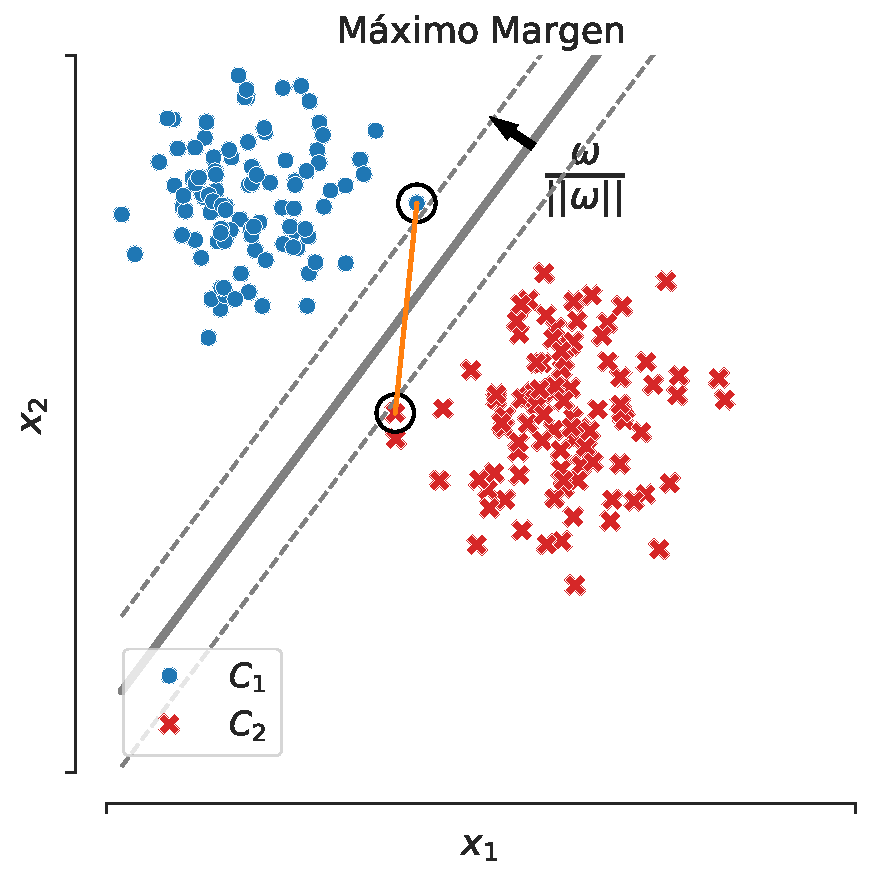
\includegraphics[width=\textwidth]{../img/cap5_max_margen2.pdf}
\end{figure}
\end{column}

\begin{column}{0.6\textwidth}

Sean $x_+\in C_1$ y $x_-\in C_{-1}$ vectores soporte, luego:
\begin{equation*}
	m = \frac{1}{2} \norm{\operatorfont{proy}_w(x_+-x_-)} =\frac{1}{2} \frac{w^\top(x_+ - x_-)}{\norm{w}}
\end{equation*}

Donde $w^\top(x_+ - x_-) = \left((1-b) - (-1-b)\right) = 2$.\\~\

Luego:
\begin{equation*}
	m=\frac{1}{||w||}
\end{equation*}

\end{column}

\end{columns} 

Para evitar problemas de diferenciabilidad, en vez de maximizar $m$, se minimizará el siguiente problema equivalente:

\begin{equation*}
\begin{aligned}
(P)\quad & \underset{w,b}{\min}
& & \frac{1}{2}||w||^2\\
& \text{s.a}
& & y_i (w^\top x_i +b) \geq 1, \; i \in\{ 1, \ldots, N\}
\end{aligned}
\end{equation*}
	
\end{frame}

\begin{frame}{SVM: formulación dual}

El problema de optimización $(P)$ cumple la restricción de Slater por lo que hay dualidad fuerte.\\~\

En este caso, el \textbf{lagrangiano} es el siguiente:

\begin{equation*}
    L(w,b,\alpha) = \frac{1}{2}||w||^2 + \sum\limits_{i=1}^{N} \alpha_i \left(1-y_i (w^\top x_i +b)\right)\label{eq:lagrangiaano_svm}
\end{equation*}

Para el \textbf{lagrangiano dual} $\theta(\alpha)=\inf_{w,b} L(w,b,\alpha)$ se utiliza CPO (ya que $L$ es convexo):

\begin{itemize}
	\item $\frac{\partial L}{\partial w} = w^\top - \sum_{i=1}^N \alpha_i y_i x_i^\top = 0 \implies \overline{w} = \sum_{i=1}^N \alpha_i y_i x_i$.
	\item $\frac{\partial L}{\partial b} = -\sum_{i=1}^N \alpha_i y_i = 0 \implies \sum_{i=1}^N \alpha_i y_i = 0$.
\end{itemize}

\vspace{.2cm}Sustituyendo:
\begin{equation*}
	\theta(\alpha) = \sum_{i=1}^N \alpha_i - \frac{1}{2} \sum_{i,j=1}^N \alpha_i \alpha_j y_i y_j \langle x_i,x_j\rangle
\end{equation*}

\textbf{Observación:} falta encontrar el parámetro óptimo $\overline{b}$.


\end{frame}

\begin{frame}{SVM: formulación dual}
	Luego, el \textbf{problema dual} $(D) \max_{\alpha\geq 0} \theta(\alpha)$  corresponde a:
	
\begin{equation*}
\begin{aligned}
(D)\quad & \underset{\alpha}{\max}
& & \sum\limits_{i=1}^{N}\alpha_i - \frac{1}{2} \sum\limits_{i,j=1}^{N} \alpha_i \alpha_j y_i y_j \langle x_i, x_j\rangle\\
& \text{s.a}
& & \sum\limits_{i=1}^{N} \alpha_i y_i= 0 \\
& &  &\alpha_i \geq 0
\end{aligned} \label{eq:dualSVM}
\end{equation*}
	
Por dualidad fuerte, si $\overline{\alpha}$ es solución de $(D)$, entonces se tiene que $\overline{w} = \sum_{i=1}^N \overline{\alpha}_i y_i x_i$	es solución para $(P)$.\\~\

Para el parámetro óptimo $\overline{b}$:

\begin{itemize}
	\item $a:=\min\limits_{i:y_i=1} \overline{w}^\top x_i \rightarrow$ distancia a la muestra más cercana (clase $1$).
	\item $b:=\max\limits_{i:y_i=-1} \overline{w}^\top x_i \rightarrow$ distancia a la muestra más cercana (clase $-1$).
\end{itemize}

Luego, se toma $\overline{b}=-\frac{a+b}{2}$.

\end{frame}

\begin{frame}{SVM: predicción}
	
Dado que se utiliza el clasificador $\overline{w}^\top x+\overline{b}=0$, para una nueva observación $x_0$, se tiene que su clase predicha es:

\begin{equation*}
 	\hat{y}_0 = \text{sign}\left(\sum\limits_{i=1}^{N} \overline{\alpha_i} y_i \langle x_i, x_0\rangle + \overline{b}\right)
 \end{equation*}
 
 Donde $\overline{\alpha}$ representa la solución del problema dual.\\~\
 
 Por otra parte, debido al teorema de holgura complementaria:
 \begin{equation*}
 	\alpha_i\left(1-y_i\left(\overline{w}^\top x_i+\overline{b}\right)\right)=0,\quad\forall i\in\{1,\ldots,N\}
 \end{equation*}
 
 Por lo tanto, si $x_i$ no es vector soporte (i.e., no está en el borde) $\implies\overline{\alpha}_i=0$. Luego:
 
 \begin{equation*}
 	\hat{y}_0 = \text{sign}\left(\sum\limits_{x_i\text{ vector soporte}} \overline{\alpha_i} y_i \langle x_i, x_0\rangle + \overline{b}\right)
 \end{equation*}
 
	
\end{frame}

\begin{frame}{Por qué usar el problema dual}

Existen distintos argumentos de por qué usar el problema dual para SVM:

\begin{itemize}
	\item El teorema de dualidad fuerte asegura que resolver el dual entregará una solución primal (en caso de existir).
	\item Las entradas $x_i$ solo interactúan en forma de productos internos.
	\item Las variables duales son indicatrices de vectores soporte y simplifica el cálculo de una predicción.
	\item El problema dual no depende de la dimensión de los datos (excepto en el producto interno).
	\item  La forma dual permitirá el uso de kernels.
	\item Existen algoritmos muy rápidos para resolver la forma dual (coordinate descent).
\end{itemize}
	
\end{frame}

\begin{frame}{Soft margin SVM}

El problema original es infactible cuando los datos no son linealmente separables. Una forma de solucionar este problema es agregar una penalización para puntos que están dentro o al otro lado del margen:

\begin{equation*}
\begin{aligned}
(P)\quad & \underset{w,b, \xi}{\text{min}}
& & \frac{1}{2}||w||^2 + c\sum\limits_{i=1}^{N} \xi_i \\
& \text{s.a}
& & y_i (w\cdot x_i +b) \geq 1 - \xi_i\\
&&&\xi_i\geq0,\; i \in\{ 1, \ldots, N\}
\end{aligned}
\end{equation*}

Donde $\xi\geq 0$ se interpretan como variables de holgura y $c>0$ es el peso entregado al regularizador $\sum\limits_{i=1}^{N} \xi_i$. En este caso, el \textbf{lagrangiano} es el siguiente:

\begin{align*}
    L(w,b,\xi,\alpha,\beta)& = \frac{1}{2}||w||^2 + c\sum \limits_{i=1}^{N} \xi_i+ \sum\limits_{i=1}^{N} \alpha_i \left(1-\xi_i -y_i (w^\top x_i +b)\right) + \sum\limits_{i=1}^{N} \beta_i(-\xi_i)\\
    & = \frac{1}{2}||w||^2 + \sum\limits_{i=1}^{N} \xi_i\left(c-\alpha_i-\beta_i\right) + \sum\limits_{i=1}^{N} \alpha_i \left(1-y_i (w^\top x_i +b)\right)
\end{align*}

 \end{frame}

\begin{frame}
	Para el \textbf{lagrangiano dual} $\theta(\alpha,\beta)=\inf_{w,b,\xi} L(w,b,\xi,\alpha,\beta)$ se vuelve a usar CPO:
	
	\begin{itemize}
	\item $\frac{\partial L}{\partial w} = w^\top - \sum_{i=1}^N \alpha_i y_i x_i^\top = 0 \implies \overline{w} = \sum_{i=1}^N \alpha_i y_i x_i$.
	\item $\frac{\partial L}{\partial b} = -\sum_{i=1}^N \alpha_i y_i = 0 \implies \sum_{i=1}^N \alpha_i y_i = 0$.
	\item $\frac{\partial L}{\partial \xi_i} =c-\alpha_i-\beta_i=0\implies \beta_i=c-\alpha_i$
\end{itemize}

Por lo tanto, el lagrangiano dual es el mismo que para hard-margin. De esta forma, el problema dual es el siguiente:

\begin{equation*}
\begin{aligned}
(D)\quad & \underset{\alpha}{\text{max}}
& & \sum\limits_{i=1}^{N}\alpha_i - \frac{1}{2} \sum\limits_{i,j=1}^{N} \alpha_i \alpha_j y_i y_j \langle x_i, x_j\rangle\\
& \text{s.a}
& & \sum\limits_{i=1}^{N} \alpha_i y_i= 0 \\
& &  & \alpha_i, \beta_i\geq 0,\quad \forall i\in\{1,\ldots,N\}
\end{aligned}
\end{equation*}
	
Y dado que $\beta_i=c-\alpha_i$, la última restricción puede escribirse como:

\begin{equation*}
	0\leq \lambda_i\leq c,\quad \forall i\in\{1,\ldots,N\}
\end{equation*}

\end{frame}


\begin{frame}{Truco del kernel}

En general, muchos algoritmos de ML, al igual que en SVM, trabajan los datos de entrada únicamente en forma de productos internos de la forma $\langle x_i,x_j\rangle$.\\~\

De esta forma, si $\phi:\R^M\to\R^D$ es un mapa de características, los datos de entrenamiento solo aparecerán de la forma $\langle \phi(x_i),\phi(x_j)\rangle$.\\~\

Estos productos internos pueden ser almacenados en una matriz (Gram matrix) $M\in\R^{D\times D}$ mediante $m_{ij}=\langle \phi(x_i),\phi(x_j)\rangle$ y así, se puede trabajar únicamente con la matriz $M$.

Por lo tanto, nace la siguiente pregunta:\\~\

Dada una función $K:\R^M\times\R^M\to\R$, ¿bajo qué condiciones $K(x_i,x_j)$ representa una matriz de productos internos?
 	
\end{frame}

\begin{frame}{Truco del kernel: teorema de Mercer}

\begin{theorem}[teorema de Mercer]

Una función continua $K: \R^M\times \R^M \to \R$ se dirá Mercer kernel si

\begin{itemize}
    \item Es simétrica: $K(x_1 , x_2 ) = K (x_2 , x_1)$
    \item Es definida positiva: para toda función $g:\R^M\rightarrow\R$ continua,
    $$\int_{\R^d\times\R^d} K(x_1, x_2)g(x_1) g(x_2) dx_1 dx_2\geq 0$$
    
\end{itemize}

Luego, si $K: \R^M\times \R^M \to \R$ es un Mercer kernel, entonces existe un espacio de Hilbert $\left(\mathcal{H},\langle,\rangle\right)$ y una función $\phi: X \to \mathcal{H}$ tal que:
	\begin{equation*}
    K(x_i, x_j) = \langle \phi(x_i) , \phi(x_j) \rangle
\end{equation*}
\end{theorem}

De esta forma, pueden sustituirse los productos $\langle x_i,x_j\rangle$ por $K(x_i, x_j)$ ya que el teorema anterior asegura que dicha evaluación representa el producto interno de los datos en algún espacio de características.

\end{frame}

\begin{frame}{Kernel SVM}
	Al sustituir los productos internos en la forma dual de SVM se obtiene el problema de \textbf{Kernel SVM}, el cual es mucho más general ya que permite separar los datos en un espacio de mayor dimensionalidad:
\begin{equation*}
\begin{aligned}
(D)\quad & \underset{\alpha}{\text{max}}
& & \sum\limits_{i=1}^{N}\alpha_i - \frac{1}{2} \sum\limits_{i=1}^{N} \alpha_i \alpha_j y_i y_j K(x_i, x_j)\\
& \text{s.a}
& & \sum\limits_{i=1}^{N} \alpha_i y_i= 0 \\
& &  &0 \leq \alpha_i \leq c
\end{aligned}
\end{equation*}

Donde $K: \R^M\times \R^M \to \R$ es un Mercer kernel asociado a algún mapa de características $\phi$ no necesariamente de dimensión finita.

\end{frame}

\begin{frame}{Ejemplos de kernels}

\begin{itemize}
	\item \textbf{Kernel polinomial:}
	\begin{equation*}
       K_{pol} (x, y) = (c + x^\top y)^d
    \end{equation*}
    donde $c\geq 0$ es un parámetro libre y $d\in\N$ es el orden del polinomio.
    \begin{itemize}
    	\item Tiene la desventaja de ser numéricamente inestable dependiendo del orden $d$.
    	\item Es muy usado en NLP con $d=2$.
    \end{itemize}
    
    \item \textbf{Kernel gaussiano (RBF): }
    \begin{equation*}
        K_{RBF} (x , y ) = \sigma^2 \exp\left(-\frac{\norm{x -y}^2}{2l^2}\right)
    \end{equation*}
    \begin{itemize}
    	\item Tiene asociado un mapa de características infinitodimensional.
    	\item Está asociado a KNN debido a que suaviza un diagrama de Voronoi.
    	\item Es el kernel por defecto en SVM.
    \end{itemize}
    
    \item \textbf{Kernel periódico:}
    \begin{equation*}
       K_{per} (x , y) = \sigma^2 \exp\left(- \frac{2\sen^2 \left(\frac{\pi|x -y|}{p}\right)}{l^2}\right).
    \end{equation*}
\end{itemize}

Además, se pueden combinar nuevos kernels sumando y/o multiplicando kernels usuales.
	
\end{frame}



\end{document}
